\documentclass[10pt,a4paper]{beamer}

\usepackage[utf8]{inputenc}
\usepackage[russian]{babel}
\usepackage[OT1]{fontenc}
\usepackage{amsmath}
\usepackage{amsfonts}
\usepackage{amssymb}
\usepackage{makeidx}
\usepackage{graphicx}
\usepackage{xcolor}

\titlegraphic{
   
\includegraphics[width=4cm]{images/sfera.jpg}
}

\author{Николай Анохин \and Михаил Фирулик}
\title{Введение в Data Science \\ Занятие 0. Знакомство}

\begin{document}

\maketitle

\logo{
    
\includegraphics[width=3cm,keepaspectratio]{images/sfera.jpg}
}

\begin{frame}{Ваши преподаватели}

\begin{itemize}

	\item Михаил Фирулик (\href{mailto:m.firulik@corp.mail.ru}{m.firulik@corp.mail.ru}\;/\;+7 916 730-97-66) \\
	\begin{itemize}
		\item руководитель отдела анализа данных в Mail.Ru Group \\
		\item многолетний опыт интеллектуального анализа данных		
	\end{itemize}

	\item Николай Анохин (\href{mailto:n.anokhin@corp.mail.ru}{n.anokhin@corp.mail.ru}\;/\;+7 903 111-44-60)\\	
	\begin{itemize}
		\item программист-исследователь в Mail.Ru Group \\
		\item более трех лет работы в области Data Mining
	\end{itemize}

\end{itemize}

\end{frame}

% *************************************************************************** %

\begin{frame}{Права и обязанности}

\begin{itemize}

	\item можно
	\begin{itemize}
		\item задавать вопросы преподавателю
		\item выносить идеи на общее обсуждение
		\item входить и выходить, не мешая коллегам
	\end{itemize}

	\item не можно
	\begin{itemize}
		\item нарушать порядок на занятии
		\item разговаривать по телефону в аудитории	
	\end{itemize}
	
	\item общение
	\begin{itemize}
		\item с преподавателем на ``Вы''
		\item с коллегами -- как удобно
	\end{itemize}
	Ваши правила?

\end{itemize}

\end{frame}

% *************************************************************************** %

\begin{frame}{План занятия}

\tableofcontents

\end{frame}

% *************************************************************************** %

\section{Какие задачи решает Data Science}

\begin{frame}{Одна (типичная) задача}

{\small Рекламная компания магазина зимней одежды: определить аудиторию}

\begin{center}
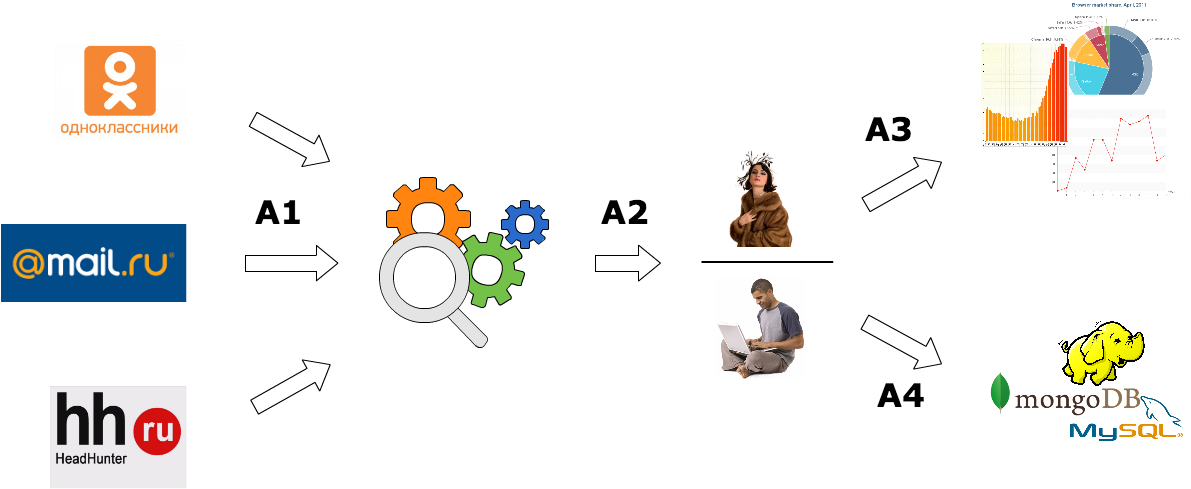
\includegraphics[scale=0.25]{images/furcoats.png}
\end{center}

\begin{itemize}
\item[A1] (data) acquisition
\item[A2] (data) analysis
\item[A3] (data) archiving
\item[A4] (data) architecture
\end{itemize}

\end{frame}

% *************************************************************************** %

\begin{frame}{Что делать?}

\begin{columns}[T]
    \begin{column}{.6\textwidth}
     \begin{block}{}
     	\begin{footnotesize}
		\begin{itemize}
		\item Разобраться в предметной области
		\item Общаться с пользователями данных
		\item Понимать ``Big Picture''
		\item Изучить представление данных
		\item Произвести подготовку и анализ данных
		\item Визуализировать результат
		\item Учитывать этические соображения
		\end{itemize}
     	\end{footnotesize}
    \end{block}
    \end{column}
    \begin{column}{.4\textwidth}
    \begin{block}{}
    \vspace{-3em}
	\begin{center}
   		
\includegraphics[scale=0.7]{images/superman.jpg}
    \end{center}
    \end{block}
    \end{column}
  \end{columns}

\end{frame}

% *************************************************************************** %

\section{Как устроен наш курс}

\begin{frame}{Мы бы хотели, чтобы вы}

\begin{enumerate}
\item получили практический опыт решения задач Data Mining
\item познакомились с инструментарием
\item поиграли и получили удовольствие
\end{enumerate}

\end{frame}

% *************************************************************************** %

\begin{frame}{Что необходимо повторить}

\begin{enumerate}
\item Линейная алгебра
\item Теория вероятностей
\item Алгоритмы и структуры данных
\end{enumerate}

\end{frame}

% *************************************************************************** %

\begin{frame}{Модули курса}

\begin{enumerate}
\item Задачи классификации (6 занятий)
\item Задачи кластеризации (3 занятия)
\item Мета-алгоритмы (4 занятия)
\end{enumerate}

\end{frame}

% *************************************************************************** %

\begin{frame}{Модуль 1. Задачи классификации}

{\bf Задача} Разработать алгоритм, позволяющий определить класс произвольного объекта из некоторго множества
\begin{itemize}
\item Каждый объект заданного множества принадлежит классу из некоторого набора
\item Дана {\it обучающая выборка}, в которой для каждого объекта известен класс
\end{itemize}

{\bf Примеры}
\begin{itemize}
\item Определение спама
\item Кредитный скоринг
\item Распознавание лиц
\end{itemize}

\end{frame}

% *************************************************************************** %

\begin{frame}{Модуль 1. Содержание}

 \begin{columns}[T]
    \begin{column}{.4\textwidth}
     \begin{block}{}
     	\begin{footnotesize}
     		\begin{enumerate}
     		\item Задача классификации и регрессии. Метрики ошибок
			\item Линейная и логистическая регрессия
			\item Решающие деревья
			\item Байесовские алгоритмы
			\item Метод опорных векторов    		
     		\end{enumerate}     				
     	\end{footnotesize}
    \end{block}
    \end{column}
    \begin{column}{.55\textwidth}
    \begin{block}{}
    \vspace{-3em}
	\begin{center}
   		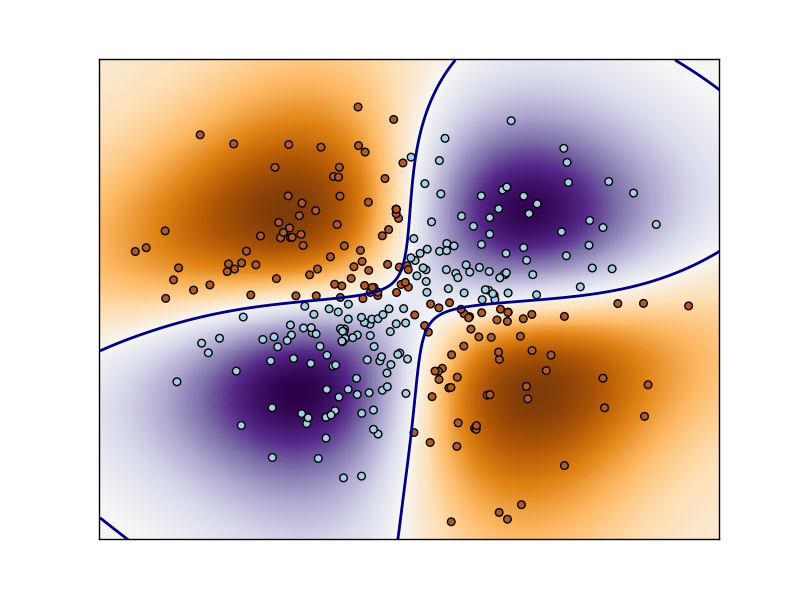
\includegraphics[scale=0.3]{images/svm.png}
    \end{center}
    \end{block}
    \end{column}
  \end{columns}
  
  {\bf Задача модуля.} Предсказание пола и возраста пользователей популярных социальных сервисов.

\end{frame}

% *************************************************************************** %

\begin{frame}{Модуль 2. Задачи кластеризации}

{\bf Задача} Разбить выборку объектов на подмножества (кластеры)
\begin{itemize}
\item Объекты внутри одного кластера должны быть похожи
\item Объекты из разных кластеров должны существенно отличаться
\end{itemize}

{\bf Примеры}
\begin{itemize}
\item Определение сообществ
\item Сегментация изображений
\item Исследование рынка
\end{itemize}

\end{frame}

% *************************************************************************** %

\begin{frame}{Модуль 2. Содержание}

\begin{columns}[T]
    \begin{column}{.4\textwidth}
     \begin{block}{}
     	\begin{footnotesize}
     		\begin{enumerate}
     		\item Задача кластеризации. Метрики качества 
			\item EM-алгоритм
			\item Различные алгоритмы кластеризации
     		\end{enumerate}     				
     	\end{footnotesize}
    \end{block}
    \end{column}
    \begin{column}{.55\textwidth}
    \begin{block}{}
    \vspace{-3em}
	\begin{center}
   		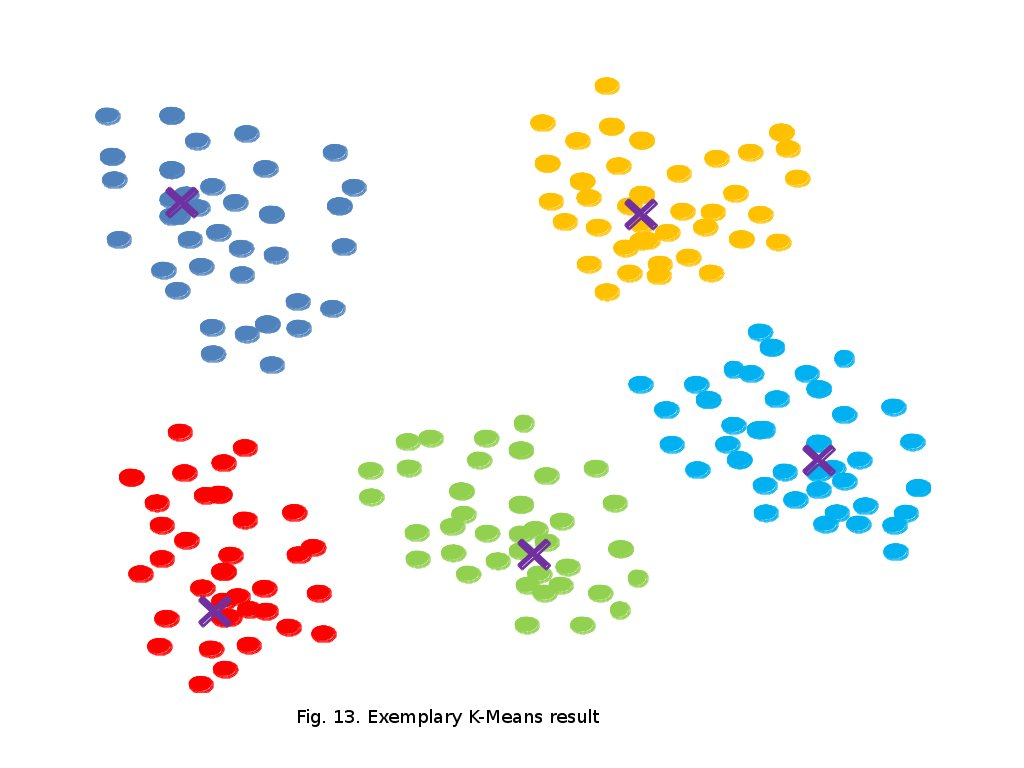
\includegraphics[scale=0.15]{images/kemans.jpg}
    \end{center}
    \end{block}
    \end{column}
\end{columns}
  
  {\bf Задача модуля.} Разбиение на категории товаров, предлагаемых крупными интернет-магазинами.

\end{frame}

% *************************************************************************** %

\begin{frame}{Модуль 3. Мета-алгоритмы}

\begin{itemize}
\item Какие факторы выбрать для решения задачи?
\item Что, если  алгоритмы не дают необходимого качества?
\item Что, если данные не помещаются в памяти?
\end{itemize}

\end{frame}

% *************************************************************************** %

\begin{frame}{Модуль 3. Содержание}

\begin{columns}[T]
    \begin{column}{.4\textwidth}
     \begin{block}{}
     	\begin{footnotesize}
     		\begin{enumerate}
     		\item Метод ансамблей
			\item Предобработка данных и выбор факторов
			\item Вычислительная модель MapReduce
     		\end{enumerate}     				
     	\end{footnotesize}
    \end{block}
    \end{column}
    \begin{column}{.55\textwidth}
    \begin{block}{}
    \vspace{-3em}
	\begin{center}
   		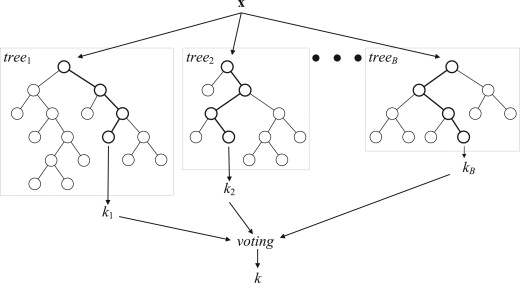
\includegraphics[scale=0.5]{images/rf.jpg}
    \end{center}
    \end{block}
    \end{column}
\end{columns}

  {\bf Задача модуля.} Классификация пользоватей интернета с использованием реальных данных сервисов Mail.Ru.

\end{frame}

% *************************************************************************** %

\section{Методология и применимость Data Science}

\begin{frame}{CRISP-DM}

\begin{center}
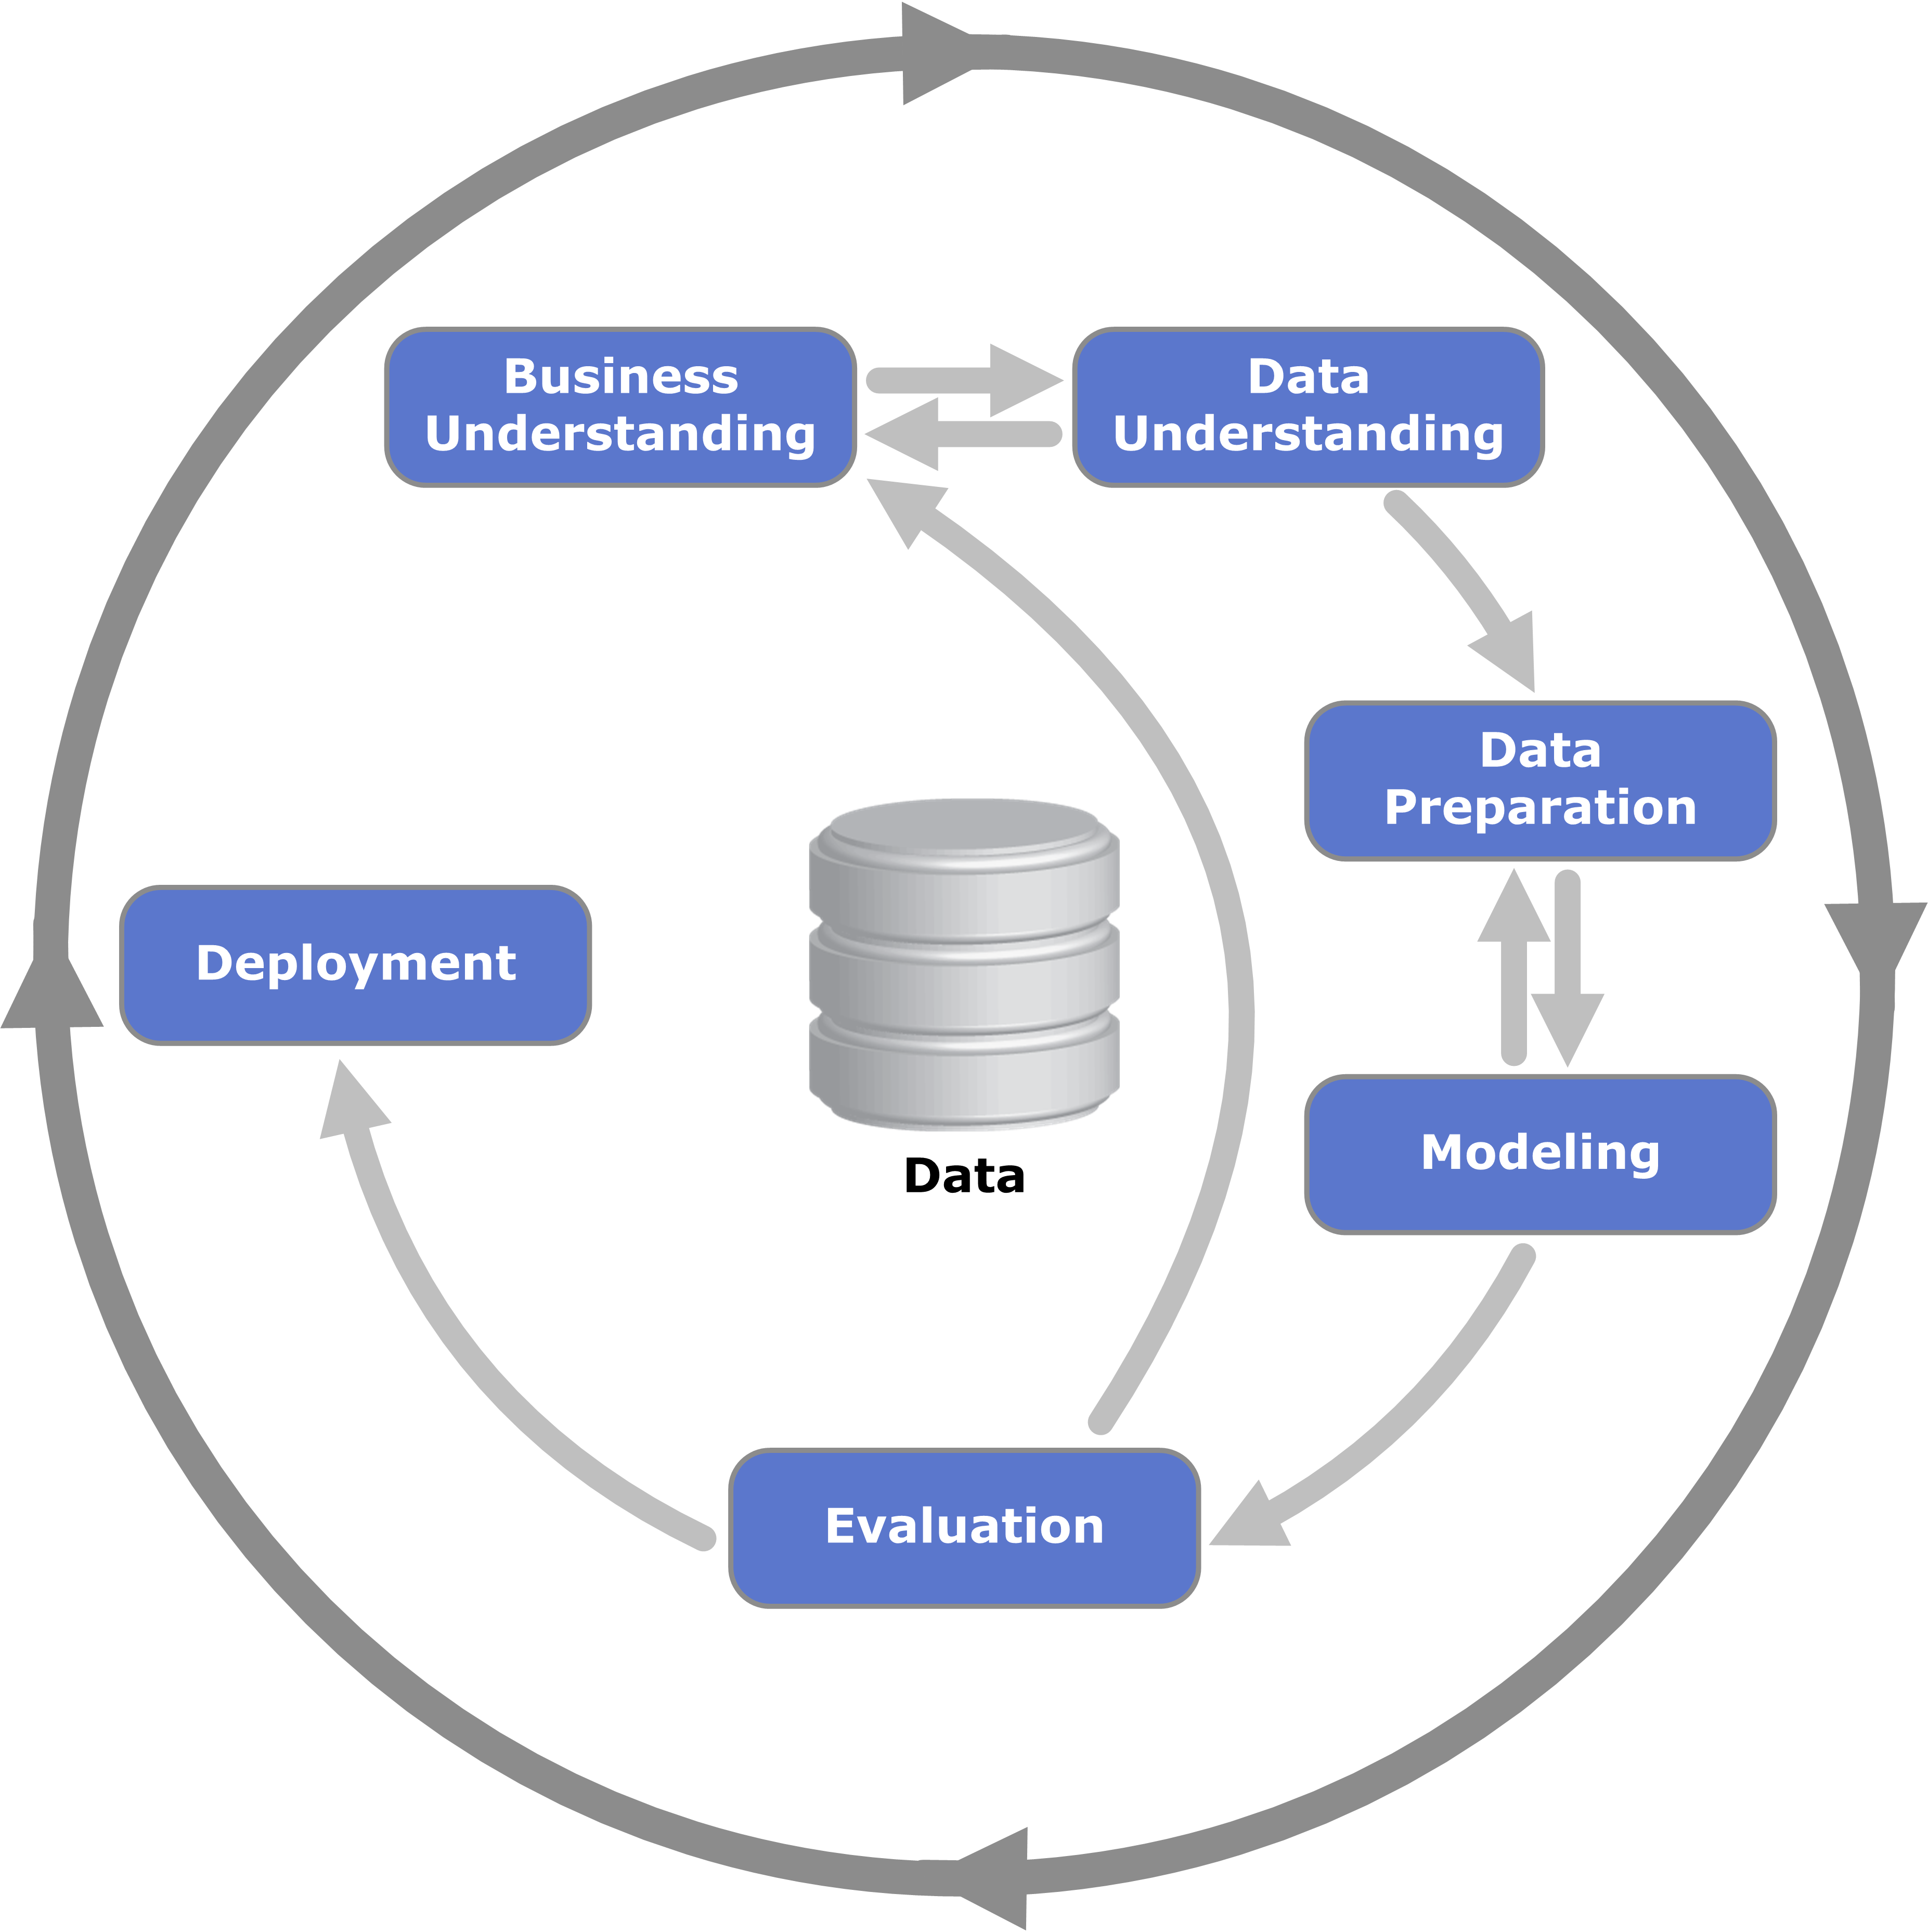
\includegraphics[scale=0.4]{images/crisp.png}

SPSS, Teradata, Daimler AG, NCR Corporation, OHRA
\end{center}

\end{frame}

% *************************************************************************** %

\begin{frame}{Business understanding}

На рыболовном предприятии автоматизируем сортировку улова

\begin{center}
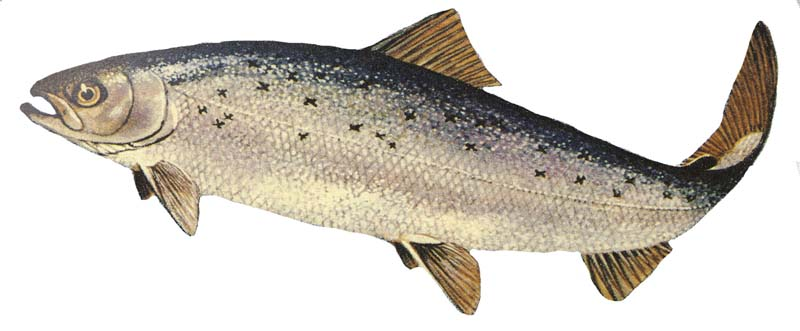
\includegraphics[scale=0.2]{images/salmon.jpg}

VS

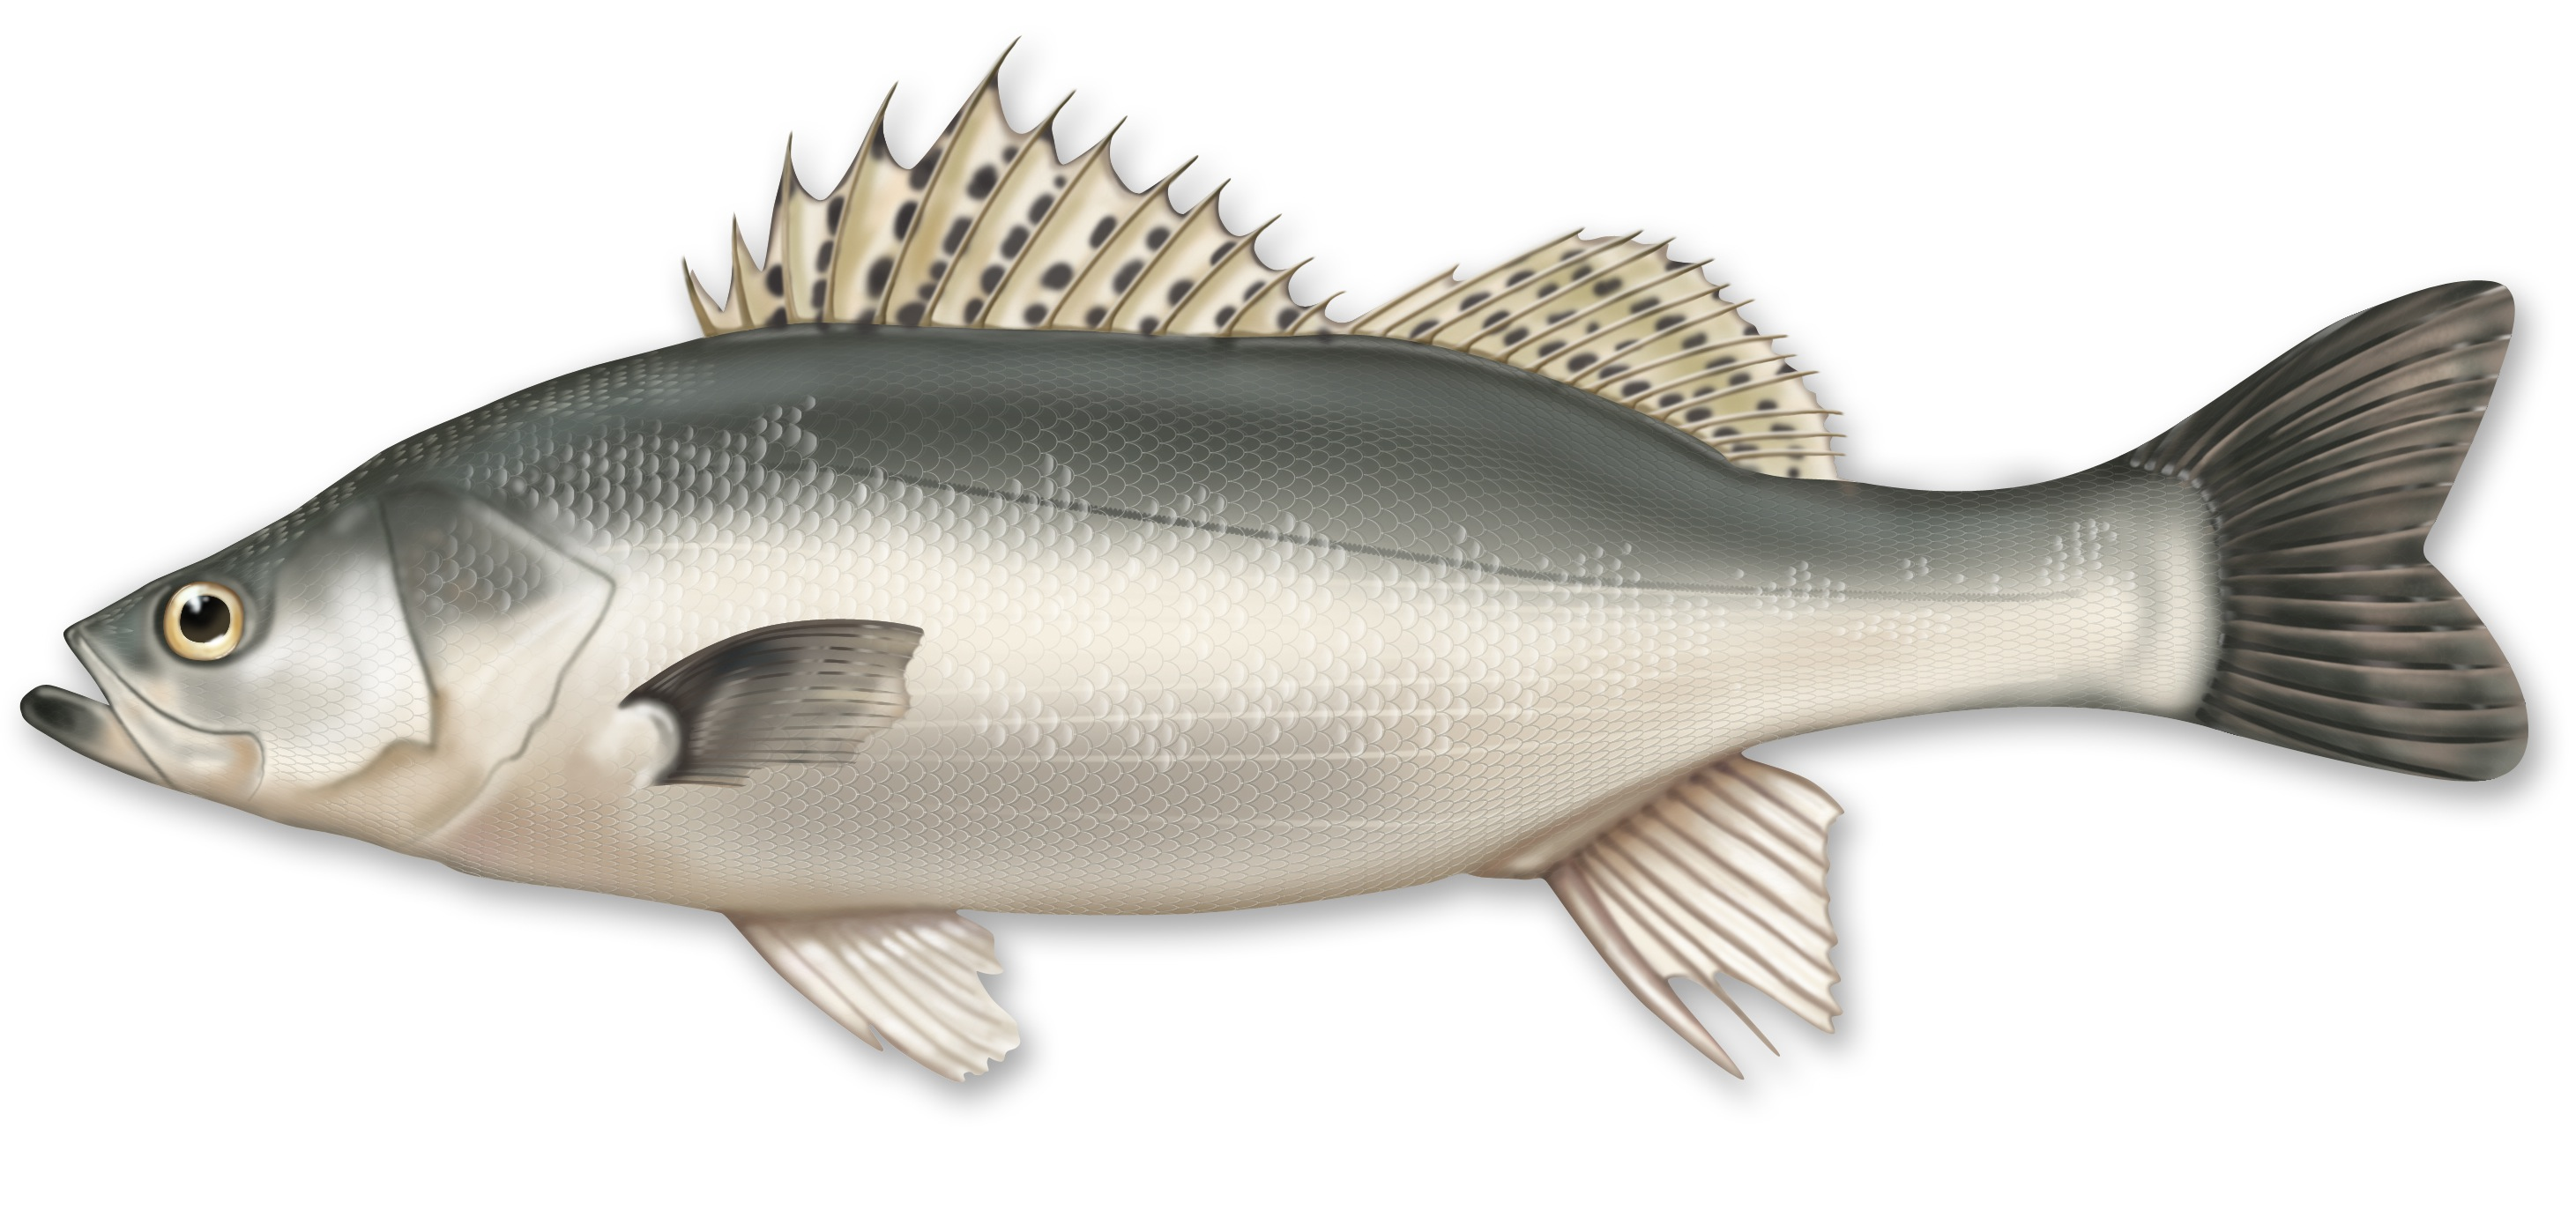
\includegraphics[scale=0.2]{images/seabass.jpg}
\end{center}

\end{frame}

% *************************************************************************** %

\begin{frame}{Data understanding 1}

Какие факторы будем использовать?

\begin{center}
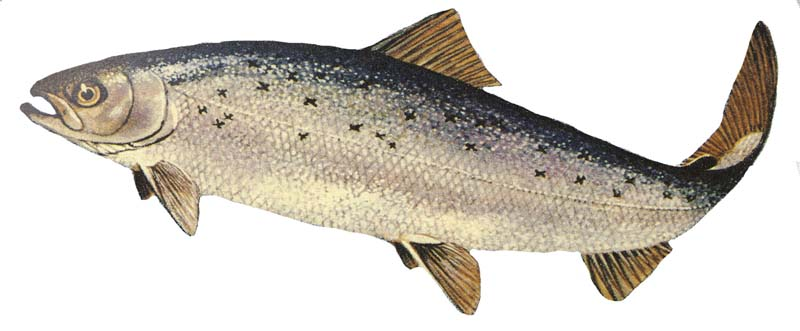
\includegraphics[scale=0.2]{images/salmon.jpg}

VS

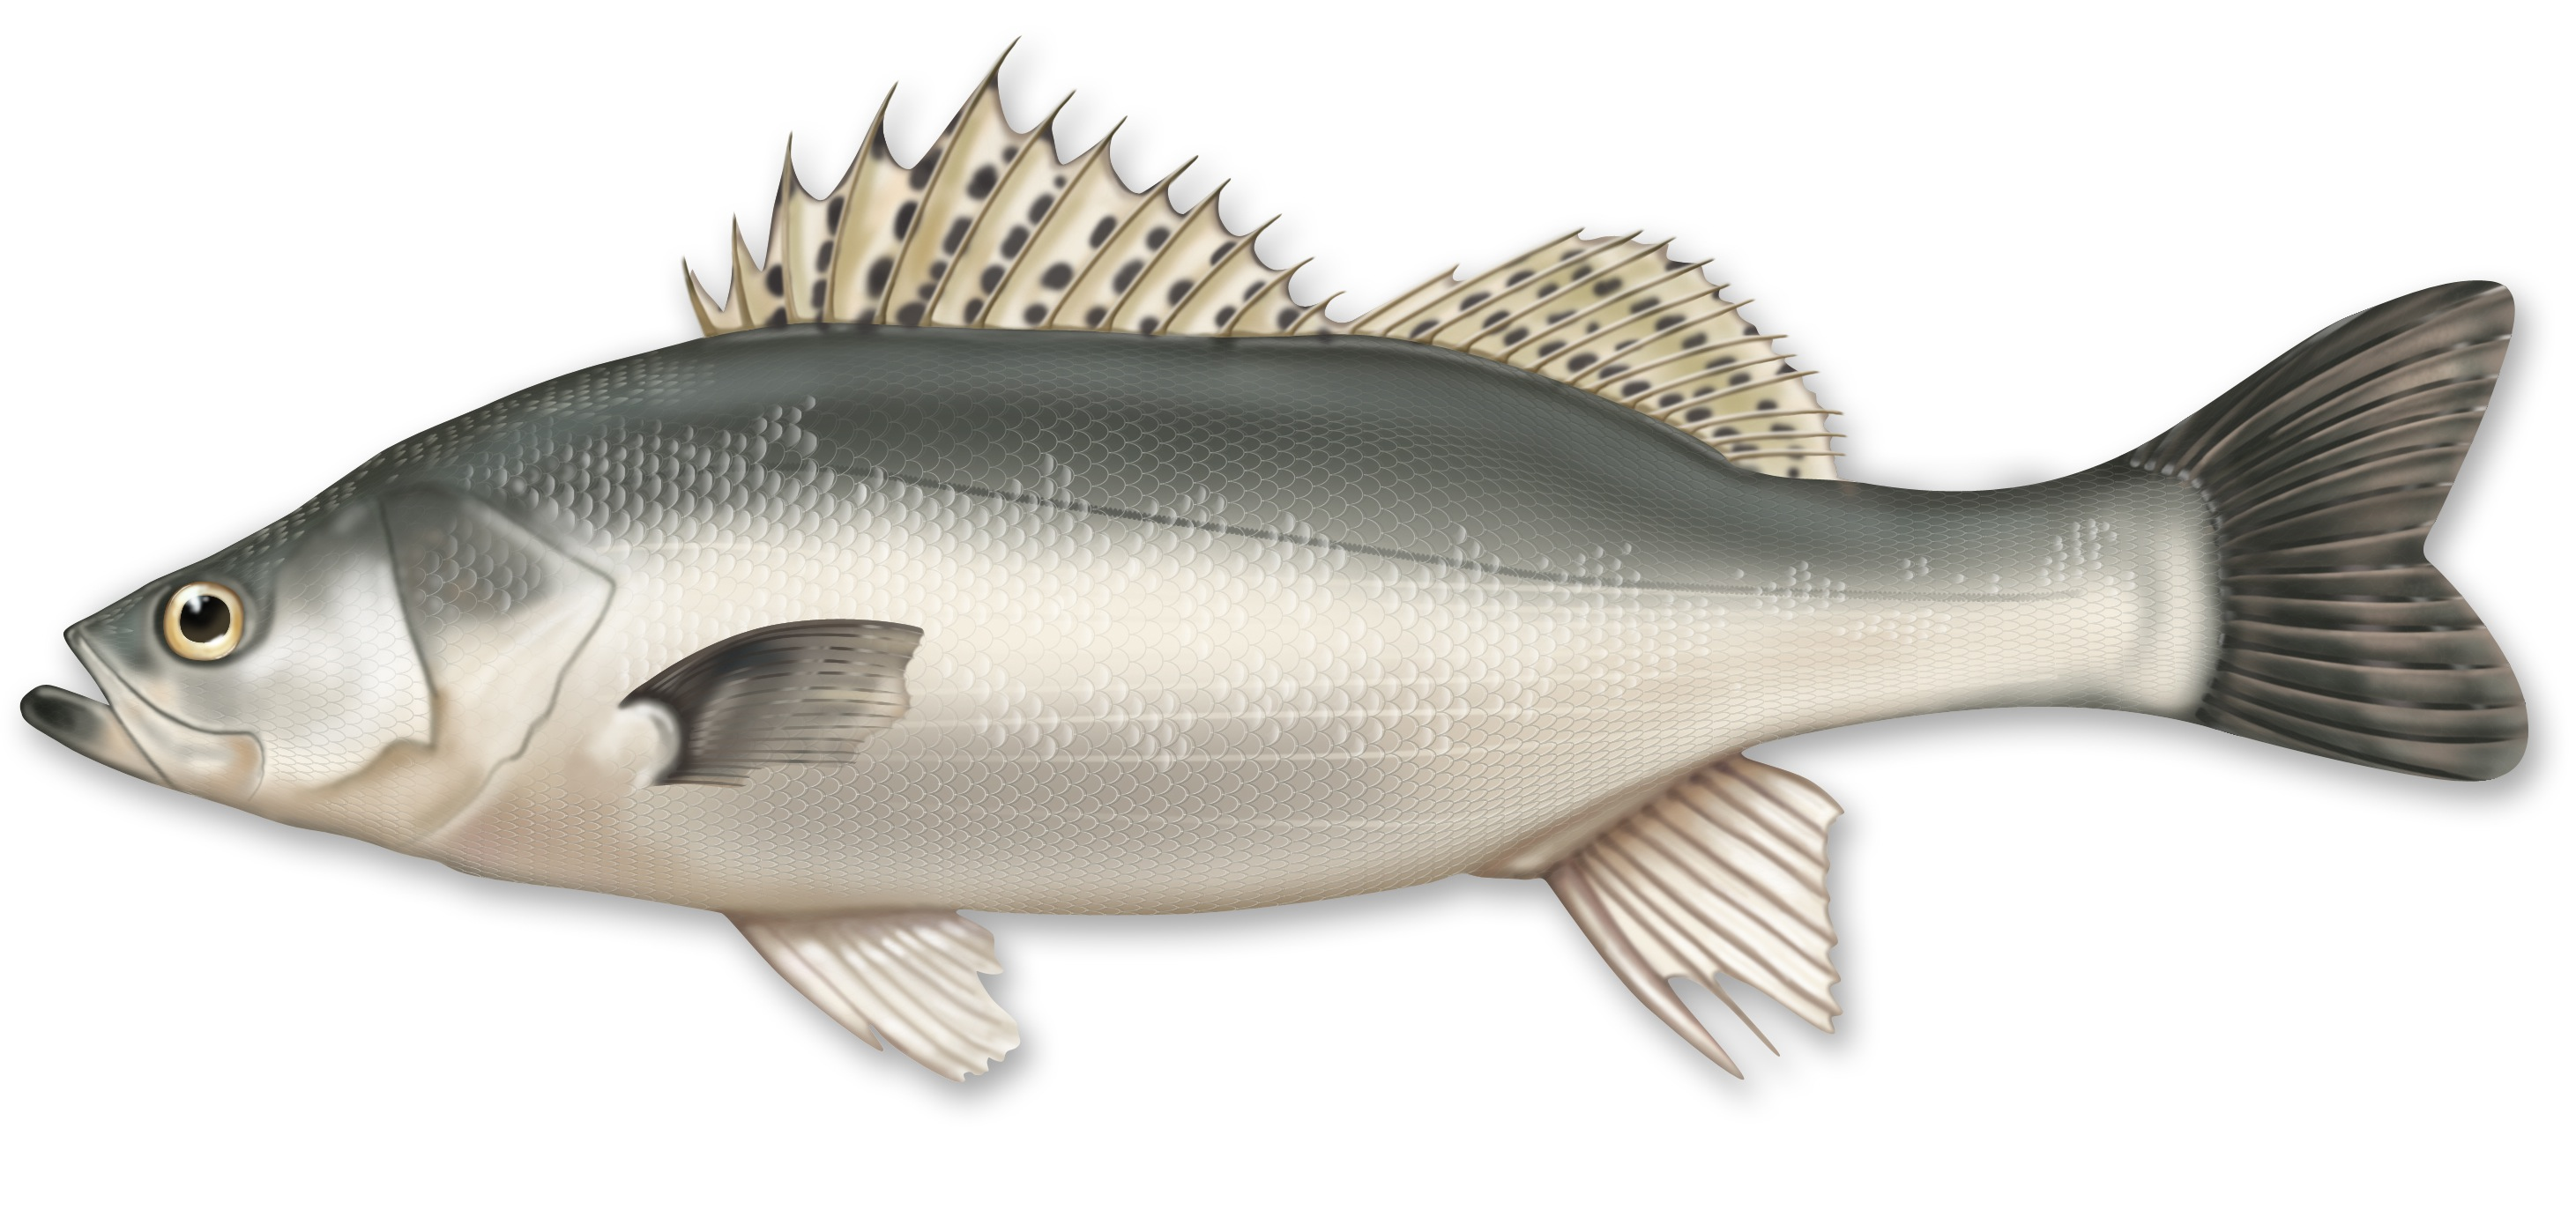
\includegraphics[scale=0.2]{images/seabass.jpg}
\end{center}

\end{frame}

% *************************************************************************** %

\begin{frame}{Data understanding 2}

$X$ -- множество объектов. Фактор $f_i: X \rightarrow F_i$

\begin{itemize}
\item Бинарные/Binary: $F_i = \{true, false\}$ (есть ли пятна, двойной ли плавник)
\item Номинальные/Categorical: $F_i$ -- конечно (цвет, форма чешуи)
\item Порядковый/Ordinal: $F_i$ -- конечно, определен порядок (категория возраста, количество плавников)
\item Количественный/Numerical: $F_i = R$ (длина, вес)

\end{itemize}

\end{frame}

% *************************************************************************** %

\begin{frame}{Data preparation}

{\bf Эта часть проекта занимает больше всего времени}

\begin{itemize}
\item Удаление шума
\item Заполнение отсутствующих значений
\item Трансформация факторов
\item Выбор факторов
\item Использование априорных знаний
\end{itemize}
{\bf Результат.} Обучающая выборка, в формате, подходящем для моделирования

\end{frame}

% *************************************************************************** %

\begin{frame}{Modeling 1}

Модель -- описание класса, выраженное, как правило, в математической форме. Цель -- выбрать удачную модель и ее параметры так, чтобы она наилучшим образом описывала заданный класс.

\begin{itemize}
\item Статистические модели
\item Модели машинного обучения
\end{itemize}

\begin{center}
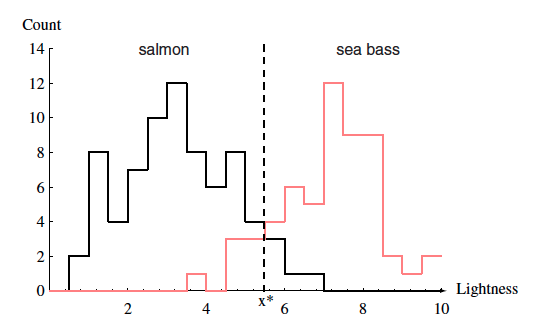
\includegraphics[scale=0.3]{images/2.png}
\end{center}

\end{frame}

% *************************************************************************** %

\begin{frame}{Modeling 2}

\begin{center}
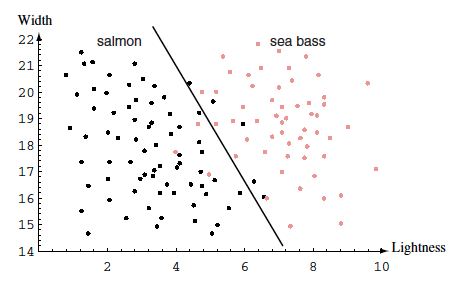
\includegraphics[scale=0.3]{images/3.png}
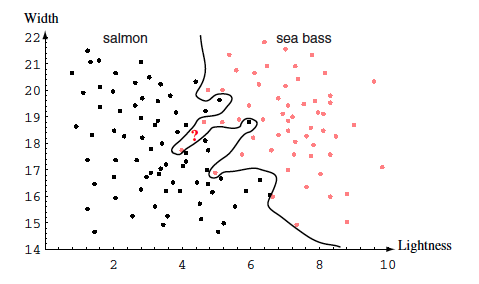
\includegraphics[scale=0.3]{images/4.png}

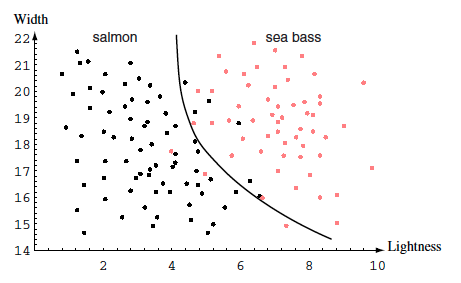
\includegraphics[scale=0.3]{images/5.png}
\end{center}

\end{frame}

% *************************************************************************** %

\begin{frame}{Evaluation \& Deployment}

\begin{itemize}
\item Решает ли выбранная модель задачу достаточно эффективно?
\item Удовлетворяет ли модель требованиям бизнеса?
\item Что вообще может пойти не так?
\end{itemize}

\begin{center}

\includegraphics[scale=0.25]{images/fail.jpg}
\end{center}

\end{frame}

% *************************************************************************** %

\begin{frame}{1854 г. Эпидемия холеры в Лондоне}

\begin{center}
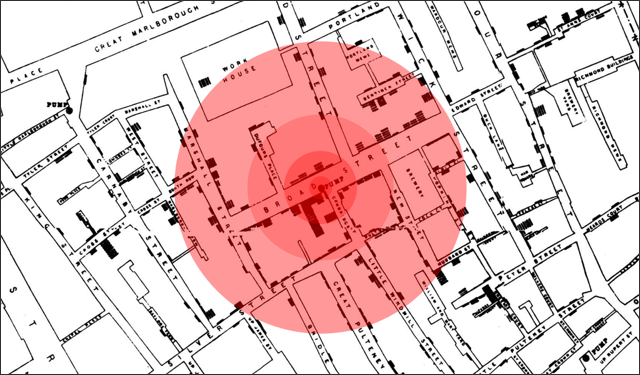
\includegraphics[scale=0.3]{images/success.png}\;
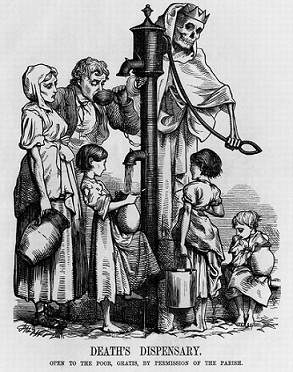
\includegraphics[scale=0.405]{images/cholera.jpg}
\end{center}

\end{frame}

% *************************************************************************** %

\begin{frame}{Программа TIA}

\begin{itemize}
\item Наблюдаем $10^9$ человек
\item Человек в среднем посещает отель раз в $100$ дней
\item Есть $10^5$ отелей на $100$ человек каждый
\item Проверим посещения за $1000$ дней 
\end{itemize}

Вероятность для конкретной пары встретиться в отеле в конкретный день:
\[
p_1 = \left(\frac{1}{100}\right)^2 \cdot 10^{-5} = 10^{-9}
\]
Всего пар людей
\[
n_{pp} = C^{10^9}_2 \approx \frac{(10^9)^2}{2} = 5 \cdot 10^{17}
\]
а пар дней
\[
n_{pd} = C^{10^3}_2 \approx \frac{(10^3)^2}{2} = 5 \cdot 10^{5}
\]
Ожидаемое количество ``подозрительных'' встреч в отелях
\[
N = p_1^2 n_{pp} n_{pd} = 250000 >> 10
\]

\end{frame}

% *************************************************************************** %

\begin{frame}{Принцип Бонферрони}

Вычислить количество рассматриваемых событий при предположении их полной случайности. Если это количество намного превосходит количество событий, о котором идет речь в задаче, полученные результаты нельзя будет считать достоверными.

\end{frame}

% *************************************************************************** %

\begin{frame}{Что мы обсудили на сегодняшней лекции?}

\begin{itemize}
\item Познакомились со стандартным процессом CRISP-DM
\item Вспомнили, какие бывают виды факторов
\item Узнали, для чего в Data Science используется моделирование
\item Разобрались с принципом Бонферрони
\end{itemize}

\end{frame}

% *************************************************************************** %

\section{Простые задачки}

\begin{frame}{Задача 1}

Пусть имеется простая обучающая выборка, включающая в себя 4 признака: бинарный $f_1$, номинальный $f_2$, порядковый $f_3$ и количественный $f_4$.

\begin{center}
\begin{tabular}{| r | c | c | c | c |}
\hline
\bf $N$ & \bf $f_1$ & \bf $f_2$ & \bf $f_3$ & \bf $f_4$ \\
\hline
\hline
1 & true & A & O1 & $3.14$ \\
2 & false & B & O2 & $2.7$ \\
3 & true & A & O2 & $11.0$ \\
4 & true & C & O1 & $10.0$ \\
\hline
\end{tabular}
\end{center}
Предложенная модель работает только на бинарных признаках. Как преобразовать данную обучающую выборку в нужный формат? А если количественный? А номинальный?

\end{frame}

% *************************************************************************** %

\begin{frame}{Задача 2}

Пусть имеется информация о покупках, совершенных 100 миллионами людей. Кажый из них идет за покупками в среднем 100 раз в год и покупает 10 из 1000 представленных товаров. Предположим, что два злоумышленника покупают одинаковые наборы товаров. Если мы ищем пары людей, купившие одинаковые наборы в течение года, сможем ли мы действительно определить террористов?

\end{frame}

% *************************************************************************** %

\begin{frame}{Спасибо!}

\begin{center}
{\Large \bf Обратная связь}
\end{center}

\end{frame}

\end{document}